% Standalone, tightly-cropped data-flow diagram for the README / landing page.
% Compile: tectonic docs/dataflow_diagram.tex  ->  docs/dataflow_diagram.pdf
% Rasterise to docs/img/dataflow.png (see scripts/render_dataflow.py).
\documentclass[border=10pt]{standalone}
\usepackage{tikz}
\usetikzlibrary{arrows.meta}

\definecolor{soft}{HTML}{555555}
\definecolor{srcblue}{HTML}{1F6FB2}
\definecolor{engamber}{HTML}{BA7517}
\definecolor{outgreen}{HTML}{3B6D11}

\tikzset{
  src/.style={rectangle, rounded corners=3pt, draw=srcblue, fill=srcblue!8, line width=0.5pt,
              align=center, text width=3.3cm, minimum height=1.3cm, inner sep=3pt, font=\footnotesize},
  proc/.style={rectangle, rounded corners=3pt, draw=soft, fill=black!5, line width=0.5pt,
               align=center, text width=7.0cm, minimum height=1.0cm, inner sep=4pt, font=\footnotesize},
  fc/.style={rectangle, rounded corners=3pt, draw=engamber, fill=engamber!10, line width=0.5pt,
             align=center, text width=6.2cm, minimum height=1.25cm, inner sep=4pt, font=\footnotesize},
  outbox/.style={rectangle, rounded corners=3pt, draw=outgreen, fill=outgreen!10, line width=0.5pt,
              align=center, text width=8.2cm, minimum height=0.9cm, inner sep=4pt, font=\footnotesize},
  lg/.style={rectangle, rounded corners=1pt, minimum width=3.2mm, minimum height=3.2mm, inner sep=0, line width=0.4pt},
  fl/.style={-{Stealth[length=2.2mm]}, draw=soft, line width=0.6pt},
}

\begin{document}
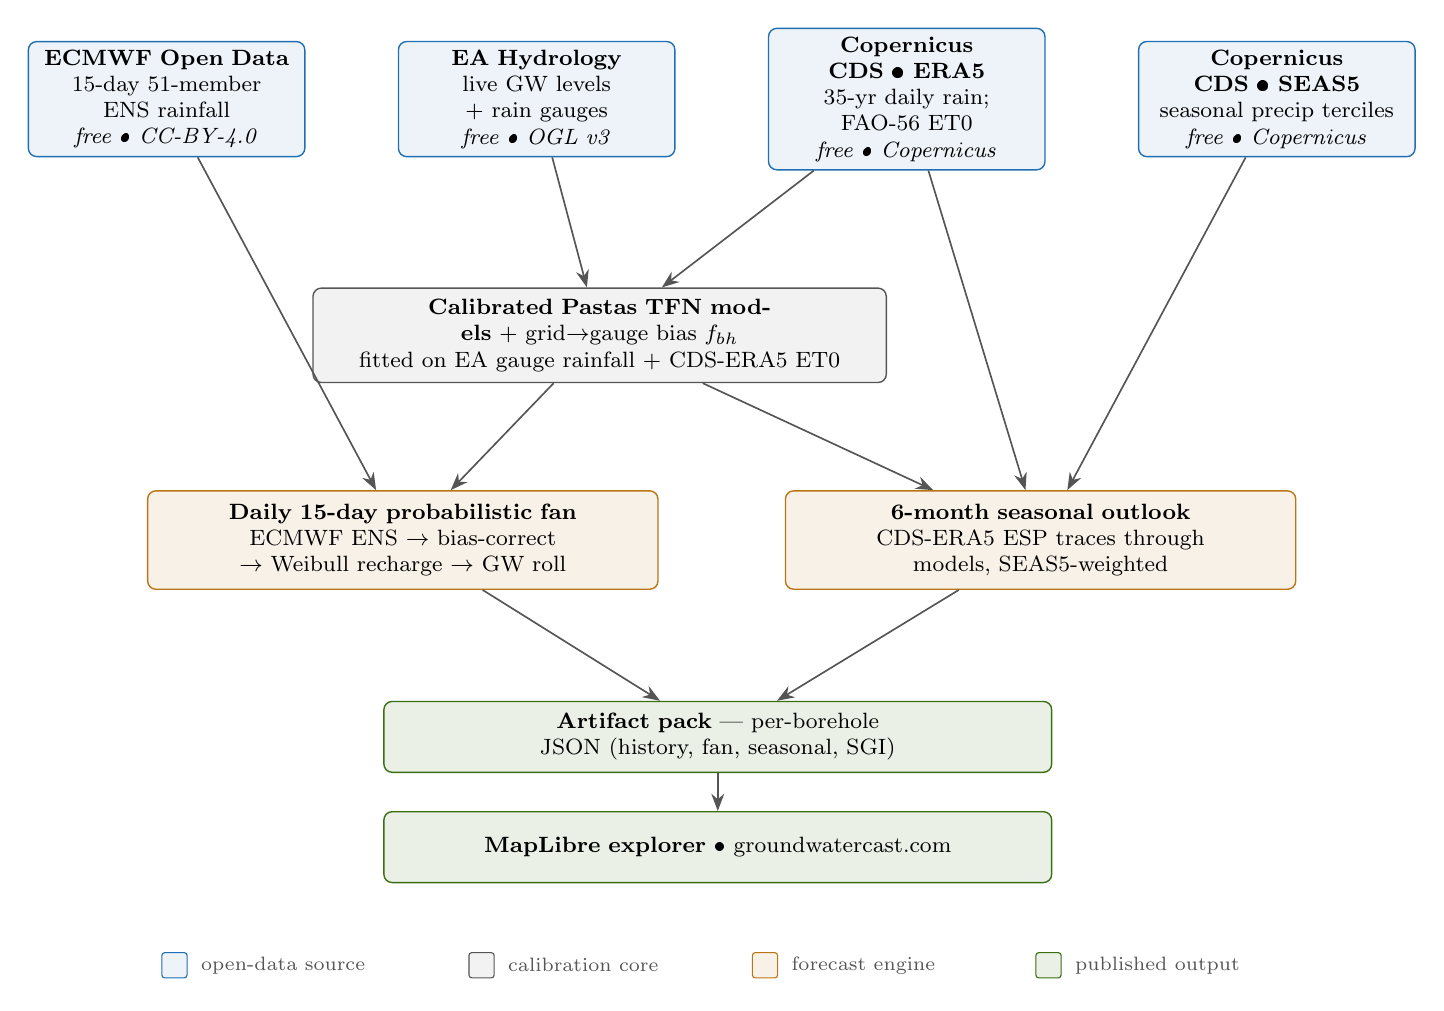
\begin{tikzpicture}
\node[src] (ecmwf) at (0,0) {\textbf{ECMWF Open Data}\\15-day 51-member ENS rainfall\\\textit{free \textbullet\ CC-BY-4.0}};
\node[src] (ea) at (4.7,0) {\textbf{EA Hydrology}\\live GW levels + rain gauges\\\textit{free \textbullet\ OGL v3}};
\node[src] (era5) at (9.4,0) {\textbf{Copernicus CDS \textbullet\ ERA5}\\35-yr daily rain; FAO-56 ET0\\\textit{free \textbullet\ Copernicus}};
\node[src] (seas5) at (14.1,0) {\textbf{Copernicus CDS \textbullet\ SEAS5}\\seasonal precip terciles\\\textit{free \textbullet\ Copernicus}};

\node[proc] (models) at (5.5,-3.0) {\textbf{Calibrated Pastas TFN models} $+$ grid$\to$gauge bias $f_{bh}$\\fitted on EA gauge rainfall $+$ CDS-ERA5 ET0};

\node[fc] (daily) at (3.0,-5.6) {\textbf{Daily 15-day probabilistic fan}\\ECMWF ENS $\to$ bias-correct $\to$ Weibull recharge $\to$ GW roll};
\node[fc] (seasonal) at (11.1,-5.6) {\textbf{6-month seasonal outlook}\\CDS-ERA5 ESP traces through models, SEAS5-weighted};

\node[outbox] (pack) at (7.0,-8.1) {\textbf{Artifact pack} --- per-borehole JSON (history, fan, seasonal, SGI)};
\node[outbox] (explorer) at (7.0,-9.5) {\textbf{MapLibre explorer} \textbullet\ groundwatercast.com};

\draw[fl] (ecmwf) -- (daily);
\draw[fl] (ea) -- (models);
\draw[fl] (era5) -- (models);
\draw[fl] (era5) -- (seasonal);
\draw[fl] (seas5) -- (seasonal);
\draw[fl] (models) -- (daily);
\draw[fl] (models) -- (seasonal);
\draw[fl] (daily) -- (pack);
\draw[fl] (seasonal) -- (pack);
\draw[fl] (pack) -- (explorer);

% legend
\node[lg, draw=srcblue, fill=srcblue!8]   (l1) at (0.1,-11.0) {};
\node[anchor=west, font=\scriptsize, text=soft] at (l1.east) {\,open-data source};
\node[lg, draw=soft, fill=black!5]         (l2) at (4.0,-11.0) {};
\node[anchor=west, font=\scriptsize, text=soft] at (l2.east) {\,calibration core};
\node[lg, draw=engamber, fill=engamber!10] (l3) at (7.6,-11.0) {};
\node[anchor=west, font=\scriptsize, text=soft] at (l3.east) {\,forecast engine};
\node[lg, draw=outgreen, fill=outgreen!10] (l4) at (11.2,-11.0) {};
\node[anchor=west, font=\scriptsize, text=soft] at (l4.east) {\,published output};
\end{tikzpicture}
\end{document}
